\section{The Prolog Language}\label{sec:the_prolog_Language}

\subsection{Brief History}\label{subsec:brief_history_prolog}
Prolog stands for \textit{PROgrammation en LOGique} and it emerged during 1970s as a way to use logic as a programming language.
The early developers of this language were Robert Kowalski, Maarten van Emden and Alain Colmelauer. The programming language, Prolog, was born of a project aimed not at producing a programming
language but at processing natural languages; in this case, French \cite{10.1145/155360.155362}. The project gave rise to a preliminary
version of Prolog at the end of 1971 and a more definitive version at the end of 1972.
Prolog gained a lot of attraction from the computing society as it was the very first logic programming language.
The language still holds considerable importance and popularity among the logic programming languages and comes with a range of commercial as well as free implementations.
\newline
Prolog is used for different kind of tasks such as:
\begin{itemize}
    \item theorem proving \cite{coelho1986automated}
    \item expert systems \cite{merritt2012building}
    \item knowledge representation \cite{gelfond2002logic}
    \item automated planning \cite{pinna2015resolving}
    \item natural language processing \cite{lally2011natural}
\end{itemize}


\subsection{Concepts}\label{subsec:concepts}
Syntax and semantics of Prolog are described in ISO standard ISO/IEC 13211. Prolog is a logic programming language; 
this means that it is used to describe known facts and relationships about a problem and less about prescribing
the sequence of steps taken by a computer to solve the problem.
When a computer is programmed in Prolog, the actual way the computer carries out the computation is specified
partially by the logic declarative semantics of Prolog, partly by what new facts can be inferred from the given ones,
and only partly by explicit control information supplied by the programmer.
\newline\newline
Prolog is used to solve problems which involve objects and relations among them.
The main features of the programming language are:
\begin{itemize}
    \item specifyng some \textit{facts} about some objects and their relationships
    \item defining some \textit{rules} about objects and their relationships
    \item asking \textit{questions} about objects and their relationships
\end{itemize}

Prolog programs are built from terms. A term is either a constant, a variable or a structure.
\subsubsection{Constants}\label{subsubsec:constants}
A constant is a sequence of characters which denotes a specific object or relationship. A constant can be an atom or a number.
All constants begin with a lower case letter.\newline\newline
\textbf{Example}\newline\newline
\textit{a} is an atom\newline
\textit{12} is a number

\subsubsection{Variables}\label{subsubsec:variables}
A variable looks like an atom except it has a name beginning with capital letter or underline signed.
A variable should be thought of as standing for some objects we are unable or unwilling to name at the time we write the program.\newline\newline
\textbf{Example}\newline\newline
\textit{X} and \textit{Answer} are valid names for variables

\subsubsection{Structures}\label{subsubsec:structure}
A structure is a collection of other objects called \textit{components}. Structures help to organize the data in a program because
they permit a group of related information to be treated as a single object instead of separate entities.
A structure is written in Prolog by specifying its \textit{functor} and its \textit{components}. The coponents are enclosed in round brackets
and separated by commas. The functor is written just before the opening round brackets.\newline\newline
\textbf{Example}\newline\newline
owns(john,book) is a structure having owns as functor and, john and book as components
\subsubsection{Facts}\label{subsubsec:facts}
A fact is a relation among objects which are all \textit{ground}. This means that a fact is a \textit{structure} which does not contain any variables among its components.
A fact is written as a structure followed by a dot (.). The names of the objects that are enclosed within the round brackets in each fact are called \textit{arguments}.
The name of the relationship which comes just before the round brackets is called \textit{predicate}.\newline\newline
\textbf{Example}\newline\newline
\textit{king(john,france)}. is a fact

\subsubsection{Rules}\label{subsubsec:rules}
A rule is a disjunction of predicates, where at most one is not negated, written in the following way:
\[ Head :- Body.\]
where Head is a predicate, Body is a conjunction of predicates and the symbol ":-" means that the body implies the head. This kind of structure is called Horn clause.
A Prolog program can be seen as a list (because order matters) of Horn clauses called \textit{theory}.
Facts could be seen as Rules having Body equals to true.
Rules are used to describe some complex relations among objects of the domain of discourse and differently from facts can contain variables.\newline\newline
\textbf{Example}\newline\newline
motherOf(X,Y) :- parentOf(X,Y),female(X).\newline\newline
The aforementioned description of Prolog language has been adapted from \cite{Clocksin1987ProgrammingIP}.

\subsubsection{Unification}\label{subsubsec:Unification}
A substitution is a function which associates a variable to a given term. The most general unifier (m.g.u.) is the substitution which allows to transform two terms making them equals
such that all other substitutions can be obtained through a composition with this one.
The unification is a process whereby two structures are made equals via substitution and it is used several times during the Prolog resolution process. 

\subsubsection{Resolution}\label{subsubsec:resolution}
The resolution in Prolog happens in the following way:the interpreter tries to verify whether a conjunction of predicates (the goal) provided by the user can be derived
from the current program or not and in the case it could, it provides a computed answer substitution (c.a.s.) which is a set of substitutions which allow to make true the user's goal.\newline
Prolog resolution process is called SLD (Selective Linear Definite clause resolution) and works as follows:\newline
SLD resolution implicitly defines a search tree of alternative computations, in which the initial goal clause is associated with the root of the tree. For every node in the tree and for every definite clause in the program whose positive literal unifies with the selected literal in the goal clause associated with the node, there is a child node associated with the goal clause obtained by SLD resolution.
A leaf node, which has no children, is a success node if its associated goal clause is the empty clause. It is a failure node if its associated goal clause is non-empty but its selected literal unifies with no positive literal of definite clauses in the program.
SLD resolution is non-deterministic in the sense that it does not determine the search strategy for exploring the search tree. Prolog searches the tree depth-first, one branch at a time, using backtracking when it encounters a failure node. Depth-first search is very efficient in its use of computing resources, but is incomplete if the search space contains infinite branches and the search strategy searches these in preference to finite branches: the computation does not terminate.
The SLD resolution search space is an or-tree, in which different branches represent alternative computations.\cite{Gallier1985LogicFC}

\subsection{2p-Kt}\label{subsec:2p_kt}

2p-Kt is a general, extensible, and interoperable ecosystem for logic programming and symbolic AI written in Kotlin which supports the Prolog ISO standard.\newline
\begin{figure}[h]
    \centering
    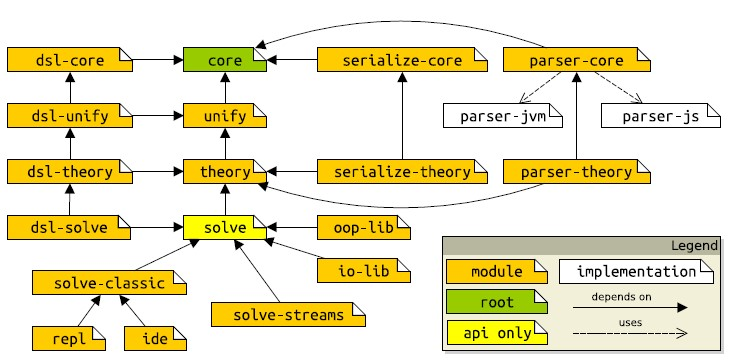
\includegraphics[width=0.70\textwidth]{images/2p_kt.jpg}
    \caption{2P-Kt project map. LP functionalities are partitioned into some loosely-coupled and incrementally-dependent modules.}
    \label{fig:2p_kt}
\end{figure}
2p-kt is the evolution of another project called tuProlog \cite{CIATTO2021100817}. To support reusability 2p-Kt is divided into several modules described as follows:
\begin{itemize}
    \item \textbf{:core}: exposes data structures for knowledge representation via terms and clauses, other than methods supporting their manipulation
    \item \textbf{:unify}: used to compare and manipulate logic terms through logic unification
    \item \textbf{:theory}: in-memory storage of clauses into ordered (e.g. queues) or unordered (e.g. multisets) data structures, and their efficient retrieval via pattern-matching
    \item \textbf{:serialize-* and :parser-*}: used to perform ancillary operations such as serialization and parsing
    \item \textbf{:solve}: aspects which are orthogonal w.r.t. any particular resolution strategy—e.g. errors management, extensibility via libraries, I/O, etc
    \item \textbf{:solve-*}: modules which implement a specific resolution strategy
    \item \textbf{:repl and :ide}: provide CLI and GUI
\end{itemize}
The structure of the project can be seen in figure \ref{fig:2p_kt}.\newline
2p-Kt provides a well-grounded technological basis for implementing/experimenting/extending the many solutions proposed in the literature—e.g., abductive
inference, rule induction, probabilistic reasoning and labelled LP.